\documentclass[11pt,border=4pt]{standalone}
\usepackage{amsmath,amssymb,bm,mathtools}
\usepackage[fontset=fandol]{ctex}
\usepackage{tikz}
\usetikzlibrary{arrows.meta,calc,patterns,angles,quotes,decorations.markings,decorations.pathmorphing}
\newcommand{\dd}{\mathop{}\!\mathrm d}
\newcommand{\e}{\mathrm e}
\tikzset{axis/.style={->,>=Stealth,line width=.45pt},world/.style={line width=.8pt},flow/.style={->,>=Stealth,line width=.7pt},ray/.style={->,>=Stealth,line width=.7pt},guide/.style={dashed,line width=.35pt},aux/.style={dashed,line width=.35pt},dim/.style={<->,>=Stealth,line width=.35pt},every node/.style={font=\small},force/.style={->,>=Stealth,very thick},gas/.style={fill=blue!7}}
\begin{document}
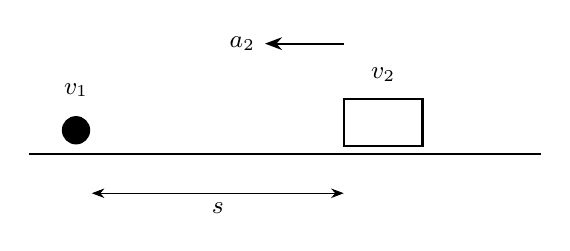
\begin{tikzpicture}\draw[world](0,0)--(6.5,0);\fill(.6,.3)circle(.18);\node[above]at(.6,.6){$v_1$};\draw[world](4,.1)rectangle(5,.7);\node[above]at(4.5,.8){$v_2$};\draw[dim](.8,-.5)--(4,-.5)node[midway,below]{$s$};\draw[flow](4,1.4)--(3,1.4)node[left]{$a_2$};\end{tikzpicture}
\end{document}
